\documentclass[../Master.tex]{subfiles}
\begin{document}




Inductive learning of STRIPS-Style actions are simple compared to actions
with conditional effect, as only objects referred to in the action parameters can be a precondition
to the effects of the action itself. However when you introduce quantifiers
then literally every object can have an effect on the outcome. Thus
our initial assumption must be that all objects in the world are 
necessary for the preconditions to be satisfied. This means for the conditional effects its quantifiers initially contains number of
variables equal to objects in the world. However by 
experiencing and seeing many different cases can we reduce it to what 
the actual number of variables and preconditions
for the conditional effects of an action are. 


\begin{figure}
	
	
	\centering{
	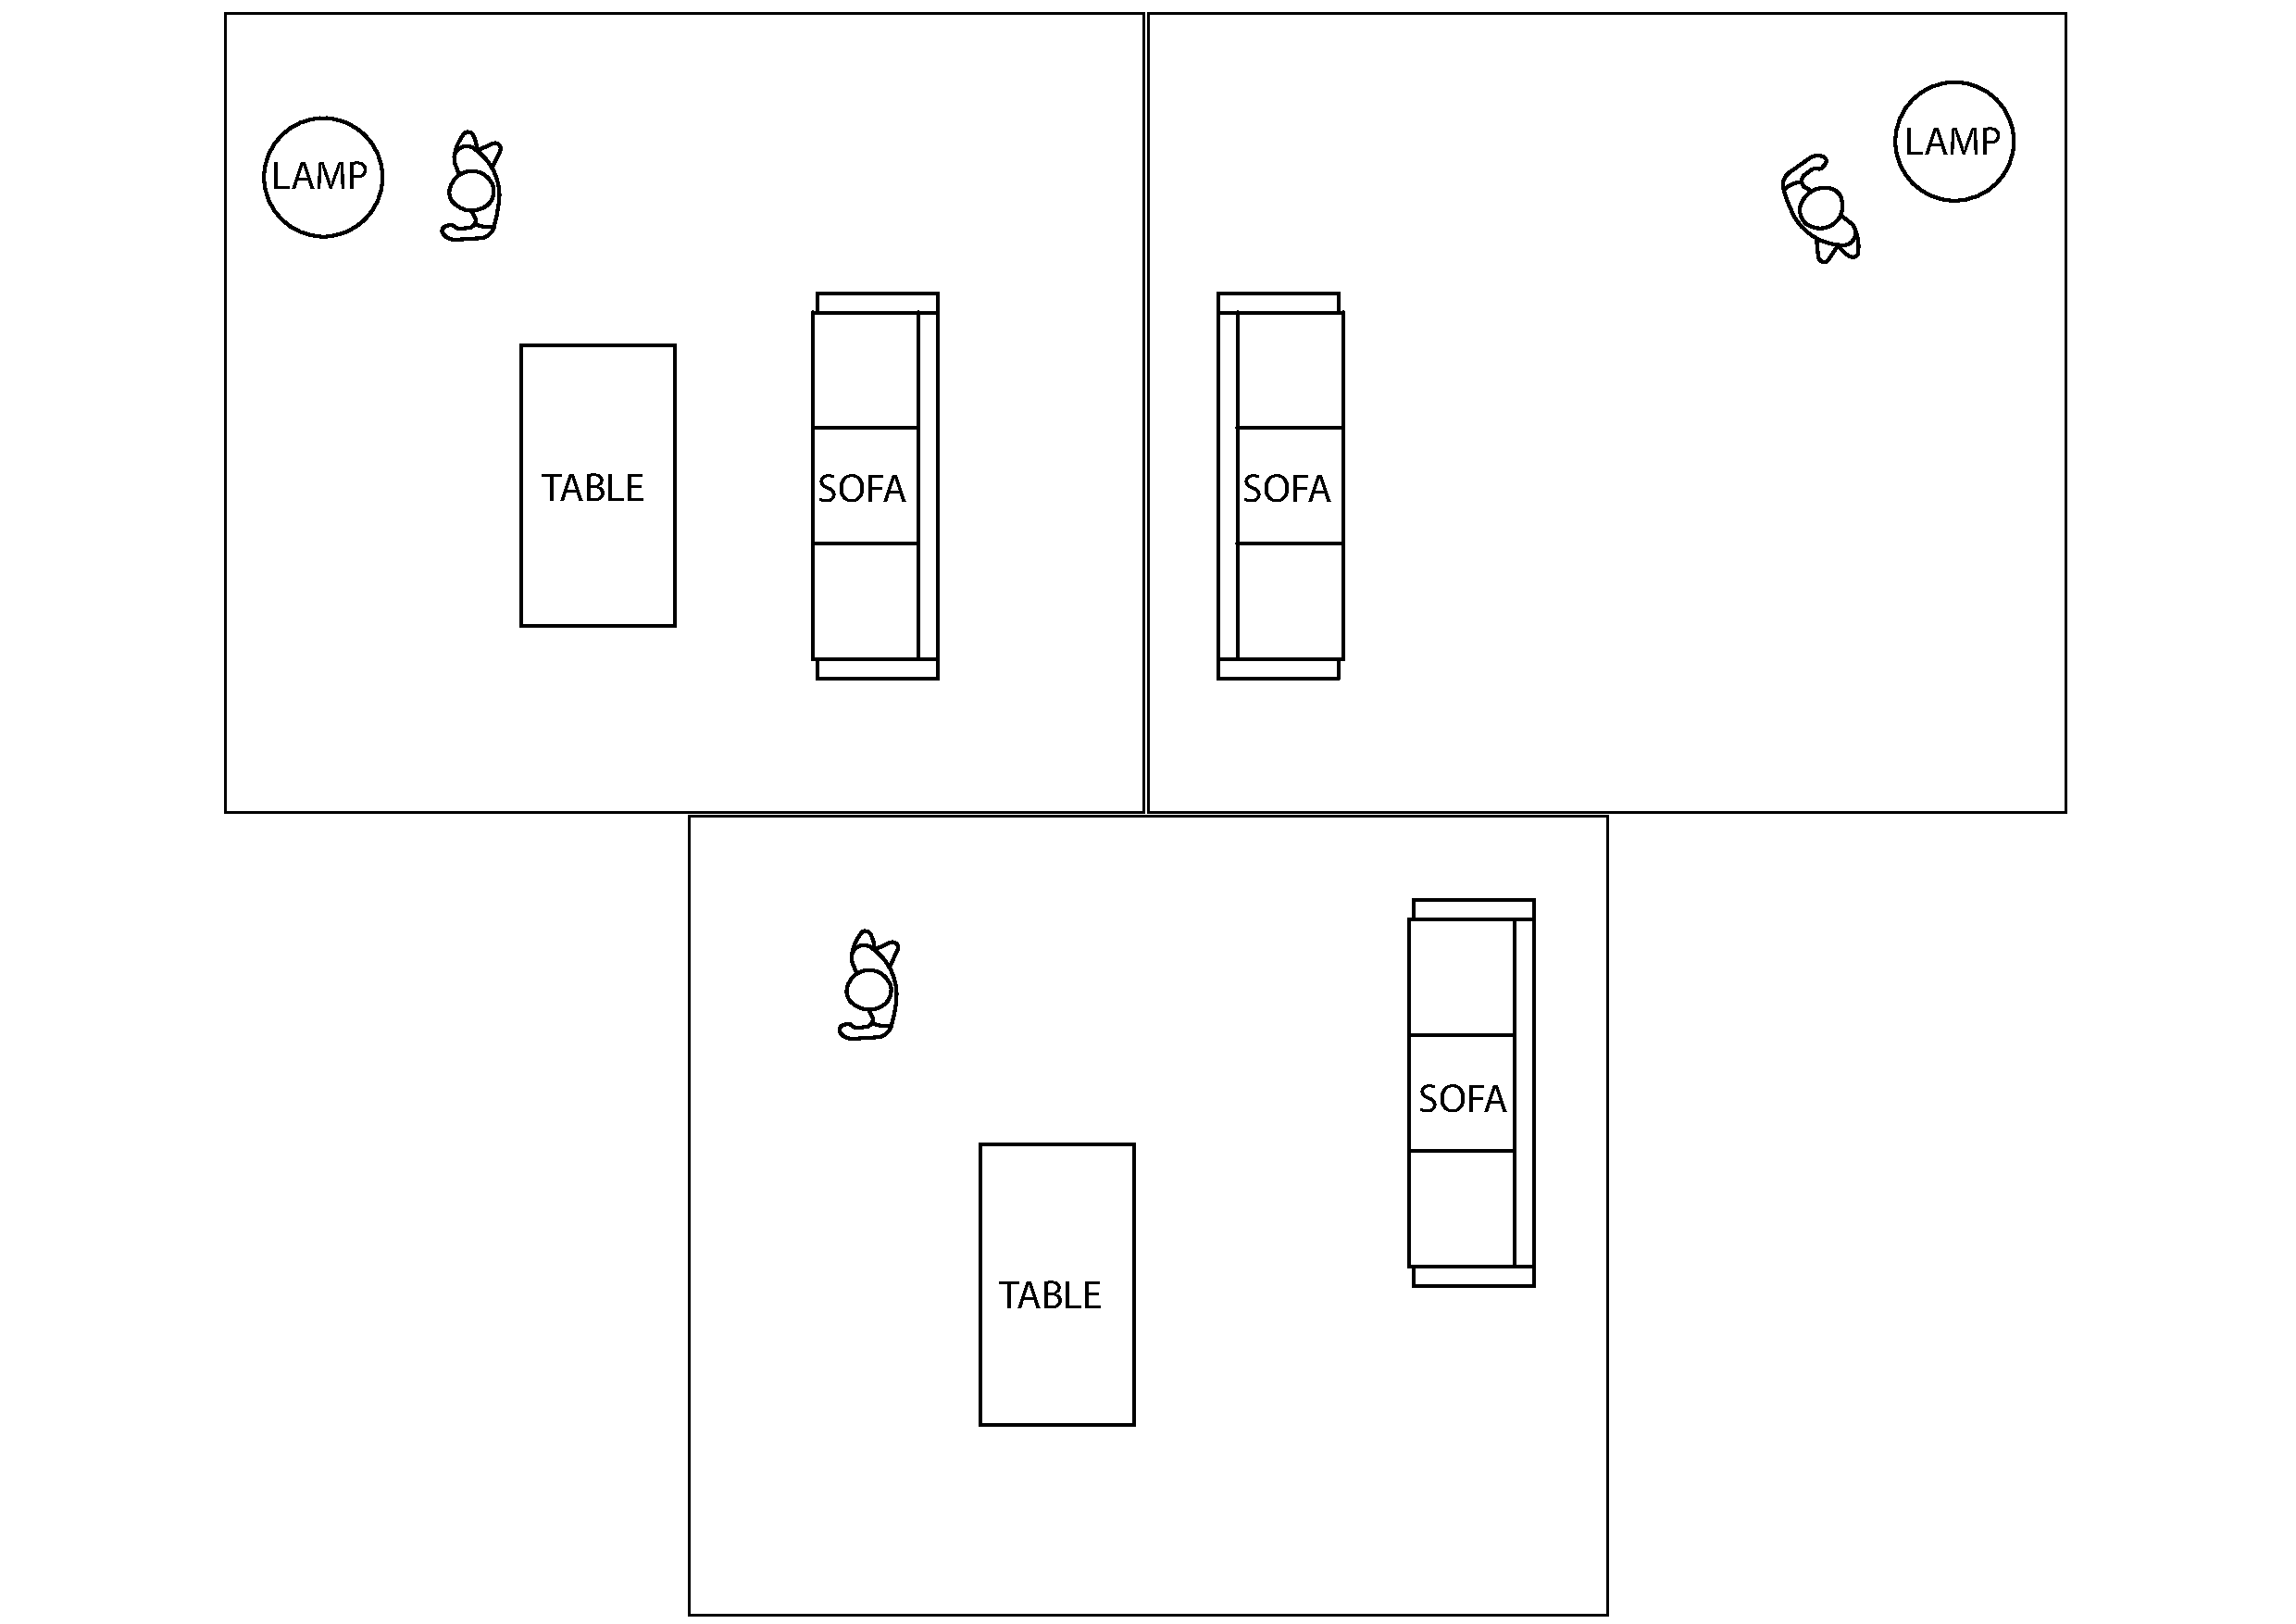
\includegraphics[width=0.5\textwidth]{../Graphics/house_conditional_knowledge.png}}
	\caption{\label{fig:House-example}Three states of light problem for Example \ref{thm:house-example}}
	
	
	
\end{figure}

\newtheorem{thm-house-example}{Example}[section]
\begin{thm-house-example}\label{thm:house-example}
Consider the problem of turning on light as shown in \figref{fig:House-example}
There in the figure there are three different cases of a person learning how to turn on the
light. In the first two cases the agent successfully turns on the light while in the last nothing occurs.

In the first case we learn the following:
\begin{itemize}
	\item A sofa in the north-east corner.
	\item A lamp in the north-west corner. With an agent on the same spot.
	\item A table in the middle.
\end{itemize}
Even though we intuitively know that it is only the lamp is the only required object in this room for the light to turn on, we cannot disprove any of the other objects presence as not being a precondition. 
\end{thm-house-example}

\subsubsection{Preconditions from states}
Objects are defined by the predicates which they satisfy. As such when we say that all objects are assumed to be required for specific effects to occur, what we are actually saying is that a specific composition of predicates is the requirement for the effects to occur.
This means that if instead see the objects as variables connecting the predicates in a pattern, then we can get an initial set of preconditions by using the state S which led to the effects.

\newtheorem{thm-precondition-state}{Theorem}
\begin{thm-precondition-state}\label{thm:precondition-state}
If an action produces one or more effects $E$, than predicates in the prior state are the maximum number preconditions to those exact effects.	

	If $\gamma (S,a) \neq S = S'$ and objects are interpreted as variables then $preconds(a) \subseteq S$  for effects $E$.
\begin{proof}[\textbf{Proof by contradiction}] Lets assume that there are more preconditions than present in S for the effects E.
	In this case the effects would not occur as their required preconditions are missing, thus the preconditions must be satisfied in S. 
	As such we can conclude S contains at least all precondition predicates.    \qedhere
\end{proof}
\end{thm-precondition-state}

\textbf{NB} For negative preconditions use $S^c$ where all predicates has been negated, as negative precondition refer to predicates not in the state. 
Thus if both negative and positive preconditions are allowed a the same time use  $S \cup \neg[S^c] $ for the preconditions.  

\begin{figure}
	\centering
	\includegraphics[width=0.2\textwidth]{../Graphics/soko_cond_example.png}
	
	\caption{\label{fig:soko-conditional}\texttt{MoveLeft} action being used in a sokoban world for Example \ref{thm:sokoban-example-initial-precond} }	
	
\end{figure}

\newtheorem{thm-sokoban-example-initial-precond}{Example}[section]
\begin{thm-sokoban-example-initial-precond}\label{thm:sokoban-example-initial-precond}
Let us consider an example of acquiring preconditions from a state modelled with predicates. In \figref{fig:soko-conditional} we see an example of an agent in the sokoban world pushing a box using a MoveLeft action with zero parameters.

The action schema that produced the effect is:
\begin{align*}
&MoveLeft():&  \\
&\quad \forall_{x, y}  \neg\texttt{at}(y) \land \texttt{at}(x) \quad when \quad \texttt{adj-h}(x,y) \land \texttt{at}(y)& \\
&\quad \forall_{x, y, z} \neg\texttt{box}(y) \land \texttt{box}(x) \quad when 
			\begin{gathered} 
				\quad \texttt{adj-h}(x,y) \land \texttt{adj-h}(y,z) \land \\ 
					  \texttt{at}(z) \land \texttt{box}(y) 
			\end{gathered}&
\end{align*}

The state transition that occurred:

\begin{equation*}\label{eq:s_before}
S_{before} =
	\left\{
		\begin{gathered}
			\texttt{adj-h}(t1, t2), \texttt{adj-h}(t2, t3), \\
			\texttt{box}(t2), \texttt{at}(t3)
		\end{gathered}
	\right\}
\end{equation*}
\begin{equation*}
S_{after} =
	\left\{
		\begin{gathered}
			\texttt{adj-h}(t1, t2), \texttt{adj-h}(t2, t3), \\
			\texttt{box}(t1), \texttt{at}(t2)
		\end{gathered}
	\right\}
\end{equation*}
The effects of the state transition we calculate:
\begin{equation*}
\Delta S =
	\left\{
		\begin{gathered}
			\texttt{box}(t1), \texttt{at}(t2), \\
			\neg\texttt{box}(t2), \neg\texttt{at}(t3)
		\end{gathered}
	\right\}
\end{equation*}
To interpret the objects as variables we provide some mapping of objects to variables, such a mapping could be:
\begin{equation*}
\delta =
	\left [
		\begin{gathered}
			t1 \mapsto x \\
			t2 \mapsto y \\
			t3 \mapsto z
		\end{gathered}
	\right ]
\end{equation*}
We apply the mapping to the objects of $S_{before}$:
\begin{equation*}
	\begin{gathered}
		\left\{
			\begin{gathered}
				\texttt{adj-h}(\delta (t1), \delta (t2), \texttt{adj-h}(\delta (t2), \delta (t3)), \\
				\texttt{box}(\delta (t2)), \texttt{at}(\delta (t3))
			\end{gathered}
		\right\} \\
		\downarrow \\
		\left\{
			\begin{gathered}
				\texttt{adj-h}(x, y), \texttt{adj-h}(y, z), \\
				\texttt{box}(y), \texttt{at}(z)
			\end{gathered}
		\right\}
	\end{gathered}
\end{equation*}
We also apply the mapping to the effects $\Delta S$
\begin{equation*}
	\begin{gathered}
		\left\{
			\begin{gathered}
				\texttt{box}(\delta (t1)), \texttt{at}(\delta (t2)), \\
				\neg\texttt{box}(\delta (t2)), \neg\texttt{at}(\delta (t3))
			\end{gathered}
		\right\} \\
	\downarrow \\
	\left\{
		\begin{gathered}
			\texttt{box}(x), \texttt{at}(y), \\
			\neg\texttt{box}(y), \neg\texttt{at}(z)
		\end{gathered}
	\right\}
	\end{gathered}
\end{equation*}

The resulting fluent predicates are the preconditions and effects 
Therefore our hypothesis of the action scheme is:
\begin{align*}
&MoveLeft_{hyp}():&  \\
&\quad \forall_{x, y, z} 
	\begin{gathered} 
		\texttt{box}(x) \land \texttt{at}(y) \land \\ \neg\texttt{box}(y) \land \neg\texttt{at}(z) \quad 
	\end{gathered}
	when 
	\begin{gathered} 
	\quad \texttt{adj-h}(x, y) \land \texttt{adj-h}(y, z) \land \\ \texttt{box}(y) \land \texttt{at}(z) 
	\end{gathered}&
\end{align*}

If our theorem is correct we should be able to use $MoveLeft_{hyp}$ on $S_{before}$ and get $S_{after}$.
\begin{align*}
&\gamma(S_{before},MoveLeft_{hyp}) = 
	\left\{
		\begin{gathered}
			\texttt{adj-h}(t1, t2), \texttt{adj-h}(t2, t3), \\
			\texttt{box}(t1), \texttt{at}(t2)
		\end{gathered}
	\right\} 
	= S_{after}
&
\end{align*}

\end{thm-sokoban-example-initial-precond}



 
\subsubsection{Initial approach to reducing preconditions}
As different scenarios are explored the unknown set $U_p$ of preconditions can be reduced.
\newtheorem{thm-unknown-set}{Definition}
\begin{thm-unknown-set}
The unknown set $U_p$ is the preconditions which has neither been proven nor disproven, initially it contains all  preconditions(universe). If an effect has been seen the $U_p$ of that is effect is equal to the state S it occurred from\footnote{Provided objects are seen as variables.} as proved in Theorem \ref{thm:precondition-state}.
\end{thm-unknown-set}
Provided that we have the $U_p$ of another state transition we can compare the two and remove discrepancies. 

As shown:

\begin{equation}
	U_p' = U_p1 \cap U_p2
\end{equation}

This will work for removing entire predicates and only if the two sets use exact same naming for variables. Herein lies the problem of reducing preconditions; unlike non-conditional effects where entire predicates are removed at a time, for conditional effects a reduction in the preconditions can simply mean the removal of a binding between two variables. 
\newtheorem{thm-binding}{Definition}
\begin{thm-binding}
	A binding between variables, means that variables between predicates are the same. 
	Bindings that contain only one variable is free and means that no binding exists. 
	It is important to note that a predicate with multiple variables can have bindings with itself.
	For instance $Q(x)$ and $P(x,y)$ has a binding on their first argument as they both refer to the same variable, and y is a free variable as no other predicates with y exists.
\end{thm-binding} 
Thus this approach to modelling the unknown preconditions, which we used for non-conditional actions is ineffective. 

\newtheorem{thm-house-example-2}{Example}[section]
\begin{thm-house-example-2}\label{thm:house-example-2}
Following from Example \ref{thm:house-example} we come to the second case in \figref{fig:House-example}
we see that we can turn on the light again but this time the sofa and the lamp has changed location and
there is no table. From this we expand our knowledge by learning:
\begin{itemize}
	\item Sofa and lamp location does not matter
	\item A table is not needed
\end{itemize}
Its important to note that since we have not seen an absence of a sofa we cannot rule out that the presence of a sofa is a precondition for the light to turn on. This is important because it shows us that by trying different scenarios we reduce the incorrect preconditions.
\end{thm-house-example-2}

\newtheorem{thm-sokoban-2}{Example}[section]
\begin{thm-sokoban-2}\label{thm:sokoban-2}
To elucidate the problem of bindings further, imagine that we have two different $U_p$
\begin{align*}
&U_p1 = \{ \texttt{p}(x, x) \} 
\end{align*}
\begin{align*}
&U_p2 = \{ \texttt{p}(x, y) \} 
\end{align*}
We see that $U_p1$ has a stronger precondition as 
\begin{align*}
&\forall_{x} \texttt{p}(x, x) \subset \forall_{x, y} \texttt{p}(x, y)  & 
\end{align*}
But if we were to take the intersection then the resulting set would be incorrect. What we actually need is to have a set of bindings and take the intersection of that.
\end{thm-sokoban-2}

\subsubsection{Idea behind proving preconditions}
Up until now we have only discussed limiting the number of possible preconditions (Unknown set) , however another aspect of learning is to determine what the actual preconditions are. 
For non-conditional actions proving the preconditions of an action was a matter of using failed actions to make a list of candidate predicates that through elimination eventually got down to just one predicate which is then proclaimed an proven precondition. The approach is similar for conditional actions however instead of having candidates of predicates conditional actions must maintain a candidate set for the bindings, and is only capable of proving a single binding at a time. 
Lets assume that we have binding set $B$
\newtheorem{thm-binding-set}{Definition}
\begin{thm-binding-set}\label{thm:binding-set}
	Binding set $B$ is a theoretical set of all bindings which differentiate between bindings from different predicates, such that the name of predicates also determines whether or not two bindings are equal. Information pertaining to the name of the variable from which the binding exists does not conflict, therefore if two $B$ sets intersected but they had completely different naming of variables than the resulting set would still be as though their name matched.
	For instance $\{p(x,x), q(x,y)\} \cap \{p(y,x), q(y,x)\} = \{p(x,y), q(x,z)\}$, notice that in they both have a binding on 
\end{thm-binding-set}
For effects that did happen in the state, the preconditions binding of shown by its prior state is then the unknown set $B_u$.
To calculate the difference between two unknown sets. Like with non-conditional effects it is:
\begin{equation}
	B_u' = B_u1 \cap B_u2
\end{equation}
If an effect did not occur in the state, the bindings in the prior state that did not produce an effect becomes the candidates $B_c$. For this set the following invariant holds
\begin{equation}
\left| \{b  |  b \in B_c \land b \in preconds_{bindings}(a)\} \right|  \ge 1
\end{equation}
Meaning that at least one of the bindings in this set is part of the bindings in the preconditions for the action $a$. As bindings that are not contained in $B_u$ is disproven to remove candidate is the same as:
\begin{equation}
B_c' = B_c \cap B_u
\end{equation}
If $|B_c| = 1$ occurs then we know that it is a correct binding and thus it is proven.

 \newtheorem{thm-house-example-3}{Example}[section]
 \begin{thm-house-example-3}\label{thm:house-example-3}
 Consider the last case on \figref{fig:House-example}. This case is identical
to the first case except it does not have a lamp, thus we learn that:
\begin{itemize}
	\item A lamp is required for the effect to occur.
\end{itemize}
Up until this transition we have not seen proof that the lamp was a precondition even though it would be intuitive for a human that still
does not mean that we can simply assume it could be that the person's action simply creates a
lamp which it then proceeds to turn on, and it was the case that no
lamp was created since it was present already.
Interestingly like with non-conditional preconditions we require failed actions to determine the actual preconditions but unlike non-conditional preconditions an action can both succeed and fail in the same step. For instance the light was successfully turned on for the lamp but it was unsuccessful in turning on the light for the sofa. 

\end{thm-house-example-3}









\end{document}
